\section{Описание раздела <<Баланс>>}
\begin{enumerate}[\thesection .1]
\item Модуль служит для просмотра списка клиентов и информации по их балансу (рис.\ref {pic:pic16_1}). В основном окне модуля отображается список клиентов, ограниченный параметрами установленных фильтров, и информация по балансу по каждому клиенту на соответствующую дату. 
\begin{figure}[!h]
	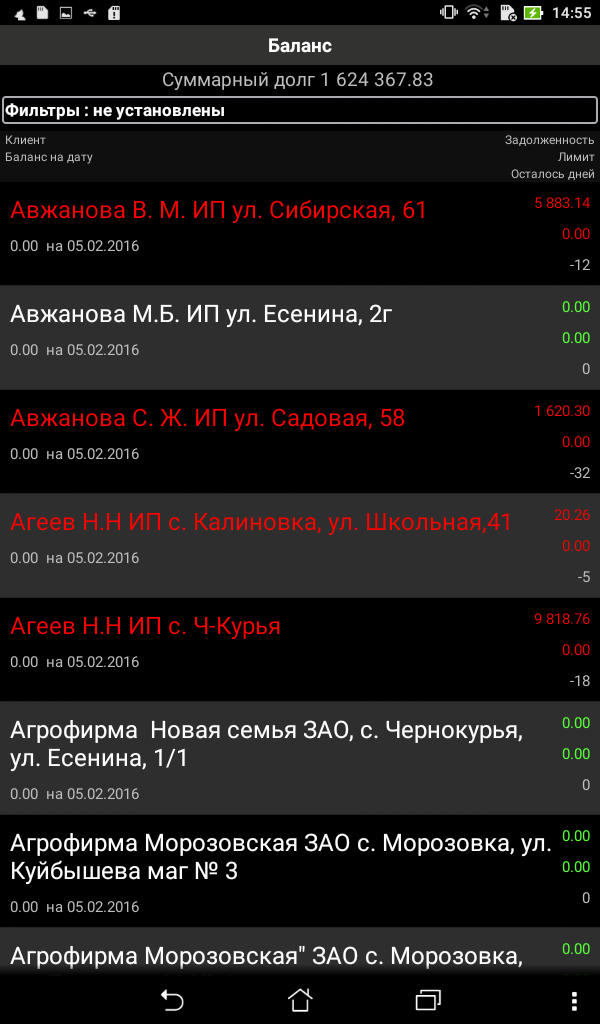
\includegraphics[width=0.4\linewidth]{scr16_1.png} 
	\caption{Баланс}\label{pic:pic16_1}
\end{figure}
Элемент списка содержит:
\begin{itemize}
	\item Наименование клиента;\footnote{Информация, отображаемая в данном поле, зависит от настроек Системы. В Системе возможно выводить в данное поле: наименование ТТ, наименование Хозяина ТТ или юр. лицо}
	\item Баланс на определённую дату;
	\item Справа от наименования клиента отображается размер задолженности клиента (в верхней строке);
	\item Кредитный лимит (в нижней строке).
\end{itemize}
Доступные фильтры:
\begin{itemize}
	\item Статус задолженности (все, без задолженности, с задолженностью и с просроченной задолженностью);
	\item Кредитное условие;
	\item Атрибут клиента;
	\item Значение атрибута клиента.
\end{itemize}
В случае если у того или иного клиента имеется просроченная задолженность,запись о таком клиенте может выделяться красным цветом. (в зависимости от настроек системы). 
%
\item Задолженность по документам
При нажатии на элемент списка в окне «Баланс» открывается окно  \textbf{(«Баланс > Подробно > Задолженности»)}. (рис.\ref {pic:pic16_2}) В данном окне отображается задолженность по оплате документов (Накладных, Накладных КИС), оформленных на выбранного клиента. 
\begin{figure}[!h]
	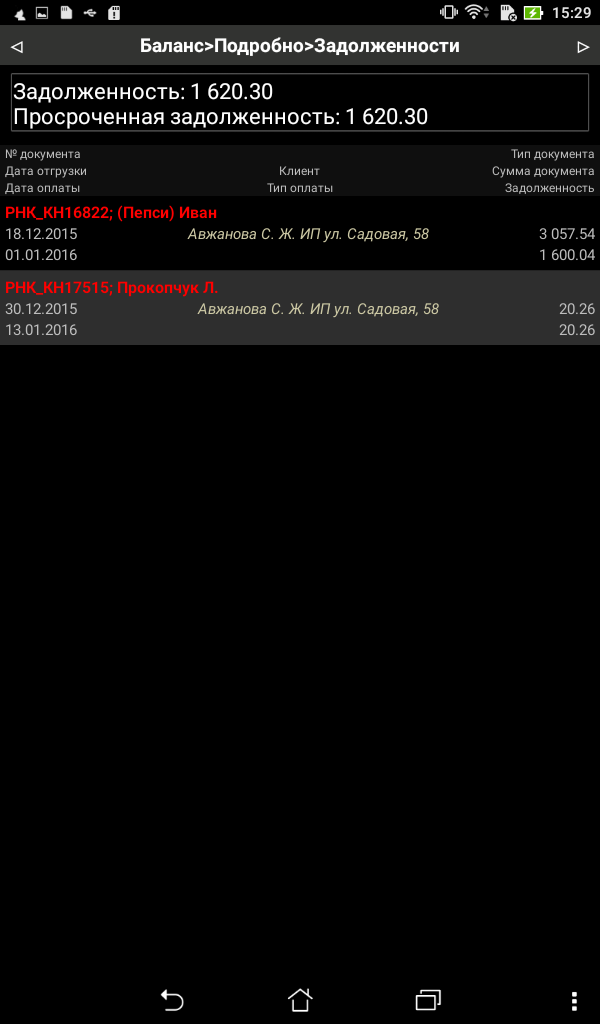
\includegraphics[width=0.3\linewidth]{scr16_2.png} 
	\caption{Задолжности}\label{pic:pic16_2}
\end{figure}
По каждому элементу списка отображается следующая информация:\footnote{Если дата оплаты документа-задолженности равна текущей дате, то номера таких документов выделяются в списке желтым цветом. Если дата оплаты документа меньше текущей даты, то номера таких документов выделяются в списке красным цветом. Остальные номера документов выделяются белым цветом.} 
\begin{itemize}
	\item № документа;
	\item Дата отгрузки – дата, на которую планируется отгрузка продукции по документу;
	\item Дата оплаты – дата, до которой клиент должен внести оплату;
	\item Клиент - наименование клиента, для которого зафиксирована задолженность;
	\item Тип оплаты – тип оплаты документа;
	\item Тип документа - тип документа, по которому зафиксирована задолженность;	
	\item Сумма документа – сумма, на которую был отгружен товар;
	\item Задолженность - сумма задолженности;	
\end{itemize}
\item История изменения баланса
Для просмотра истории изменения баланса выполните следующие действия: 
\begin{itemize}
	\item Нажмите на элемент списка в окне «Баланс»;
	\item В открывшемся окне \textbf{«Баланс > Подробно > Задолженности»} выполните скользящее касание справа – налево. Откроется окно \textbf{«Баланс > Подробно > Документы»};
\end{itemize}
В данном окне отображается история изменения задолженности выбранного клиента. Выводится список документов, повлиявших на текущую задолженность. По каждому элементу списка отображается следующая информация: 
\begin{itemize}
	\item № документа;
	\item Дата документа;
	\item Сумма - сумма по документу;
	\item Тип документа - краткое наименование типа документа;
	\item Баланс;	
\end{itemize}
%\item Баланс юридического лица
%Для просмотра информации о балансе юридического лица клиента выполните следующие действия: 
%\begin{itemize}
%	\item Нажмите на элемент списка в окне «Баланс»;
%	\item В открывшемся окне \textbf{«Баланс > Подробно > Задолженности»} выполните скользящее касание слева – направо. Откроется окно \textbf{«Баланс > Подробно > Юр. лица»}; 
%\end{itemize}
%В окне доступен фильтр по кредитному условию. По каждому элементу списка отображается следующая информация: 
%\begin{itemize}
%	\item Дата документа;
%	\item Баланс;
%	\item Задолженность – сумма задолженности;
%	\item Лимит;	
%\end{itemize}
\end{enumerate}